\documentclass{report}
\usepackage{filecontents}

\usepackage[utf8]{inputenc}
\usepackage[T1]{fontenc}
\usepackage[francais]{babel}
\usepackage{listings}
\usepackage[a4paper]{geometry}
\usepackage{graphicx}
\usepackage[export]{adjustbox}
\usepackage{titlesec}
\usepackage{color}
\usepackage[toc, page]{appendix}
\usepackage{url}

\definecolor{xcodekw}{rgb}{0.75, 0.22, 0.60}
\definecolor{xcodestr}{rgb}{0.89, 0.27, 0.30}
\definecolor{xcodecmt}{rgb}{0.31, 0.73, 0.35}

\titleformat{\chapter}[display]
  {\centering\normalfont\huge\bfseries}
  {\chaptertitlename\ \thechapter}
  {20pt}
  {\Huge}

\geometry{hscale=0.75,vscale=0.85,centering}

\renewcommand{\thesection}{\arabic{section}}
\renewcommand\appendixtocname{Annexes}
\renewcommand\appendixname{Annexes}
\renewcommand\appendixpagename{Annexes}

\title{Intégration des Technologies\\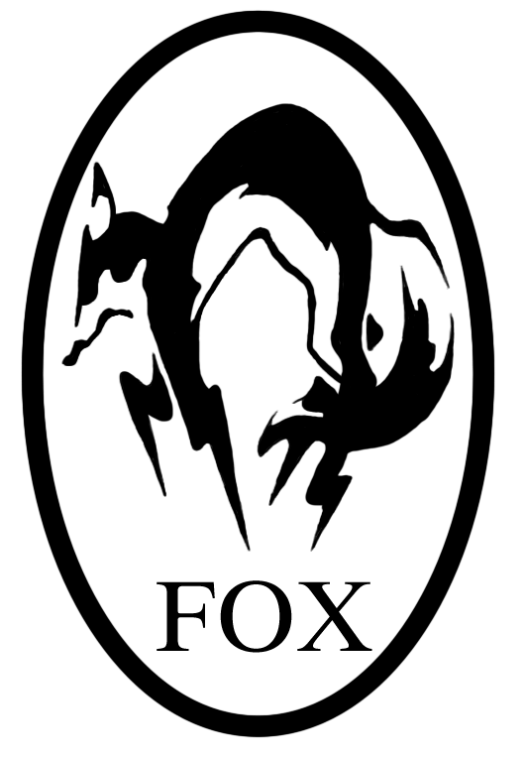
\includegraphics[scale=0.3]{foxhound.png}}
\author{Samuel "Big Boss" \bsc{Monroe}}

\date{30 Mai 2015}

\begin{document}

\maketitle

\newpage
\thispagestyle{empty}
\mbox{}

\tableofcontents

%% \textbf{}

\chapter{Avant-propos}

	Toi, mauvais élève qui n'a jamais été aux cours de Mr. Thiry, avais sans doute comme seul choix d'étudier des slides un peu austères pour l'examen.\\

	En bonne âme, je viens à toi avec cette synthèse d'une pureté ultime afin de te sauver de ton funeste destin.\\
	Composée de ce que j'ai retenu, complété via l'aides des internets, et corrélées avec les informations d'autres membres de la F0X.\\

	En espérant que tu sois membre de la F0X en mettant les mains sur ce document.\\

\chapter{Historique}

	\section{Le Chaos - 1960}

		L'historique des méthodes organisationnelle présenté ici naît avec l'apparition de l'informatique mais plus spécifiquement des langages de programmation, qui signifient que l'on va pouvoir mettre sur pied des projets de développement logiciels pour couvrir les nouveaux besoins d'applications de l'entreprise.\\

		Dans les alentours de 1960 on pourra citer le \textbf{FORTRAN} en 1954, le \textbf{COBOL} en 1959 et enfin le \textbf{BASIC} en 1964.\\

		Tout ceci étant relativement nouveau, chaque entreprise s'organise selon sa propre conception sur base des \textbf{échéances}, du \textbf{budget} ou encore de la \textbf{taille du projet}.\\

		La période de Chaos des gestions de projets est comme son nom peut le faire comprendre, une période d'\textbf{échec} sur cette gestion.

	\section{Waterfall - 1970}

		Pour pallier à cette période de Chaos un pionier du développement logiciel et scientifique informatique Américain, \textbf{Winston W. Royce}, va mettre au point le modèle \textbf{Waterfall} pour définir une manière de manager le développement de larges logiciels.\\

		Sa méthode est calquée sur ce qui se fait dans l'industrie en Amérique, qui met en avant la \textbf{planification} du projet et la maximisation de l'\textbf{éfficacité} dans chacun des maillons d'une chaîne de production.\\

		Ce modèle est nommé \textbf{Waterfall} car représente une cascade où vont se succéder : \\

		\begin{itemize}
			\item \textbf{Requirements} : On documente les besoins et les spécifications du produit.
			\item \textbf{Design} : Modélisation de l'architecture du logiciel
			\item \textbf{Implémentation} : Le développement en lui-même
			\item \textbf{Vérification} : Tests, vérification du bon fonctionnement
			\item \textbf{Maintenance}\\
		\end{itemize}

		Cette méthode va se révéler un \textbf{échec}, entraînant un système de bureaucratie contre-productif et une perte de motivation chez les acteurs du projet.\\

	\section{Lightweight - 1990}

		Les méthodologies légères vont conduire à l'émergence de méthodologies plus spécifiques apparentées que l'on développera juste après.\\

		\textbf{Lightweight} apprenant des erreurs de Waterfall va proposer une nouvelle façon d'organiser cette gestion de projets : \\

		\begin{itemize}
			\item \textbf{Pas de prédictions} : La planification à l'extrême chez Waterfall n'a pas fonctionné.
			\item \textbf{Adaptif} : Les changements étant inévitables, et ayant justement conduit à arrêter de tout prévoir, il faut à ce qu'il y aie des changements, les accepter et les gérer éfficacement.
			\item \textbf{Centré sur les gens} : Waterfall ayant cloisonné les rôles et fait perde la motivation aux acteurs, on va se recentrer sur les gens et travailler avec eux plutôt que de se concentrer sur le process.
			\item \textbf{Pas de documentation exagérée}, conduisant à la bureaucratie, à des marges de manoeuvres limitées et probablement à la perte de motivation.\\
		\end{itemize}

		\subsection{Crystal - 1992}

			Cette famille de méthodologies à été développée par \textbf{Allistair Cockburn} dans le milieu des années 90.\\

			Les méthodologies Crystal sont centrées sur les gens, leur interaction, la communauté, les compétences et talents et la communication.\\

			Ces méthodologies sont faciles d'adoption.\\

		\subsection{DSDM - 1994}

			\textbf{D}ynamic \textbf{S}oftware \textbf{D}evelopment \textbf{M}ethod, consortium créé par des vendeurs et experts, est une compilation de bonnes pratiques dans la gestion de projets.\\

			\textbf{DSDM} s'appuie sur 9 principes de bases : \\

			\begin{enumerate}
				\item Implication des utilisateurs dans le cycle de développement
				\item Autonomie
				\item Visibilité du résultat
				\item Adéquation
				\item Développement itératif
				\item Réversibilité
				\item Synthèse
				\item Tests
				\item Coopération
			\end{enumerate}

		\subsection{SCRUM - 1995}

			Métaphore liée à la mêlée du rugby utilisée pour la première fois dans une publication Japonaise de Hirotaka Takeuchi et Ikujiro Nonaka dans le monde industriel.\\

			Cette publication va inspirer \textbf{Ken Schwaber} et \textbf{Jeff Sutherland} dans ce que deviendra la méthode SCRUM.\\

		\subsection{Rational Unified Process (RUP) - 1996}

			Donne un cadre au développement logiciel avec un grand nombre de variantes pas seulement agiles.\\

			Fournit un ensemble d'outils décrivant les processus et pratiques à mettre en place pour gérer un projet.\\

		\subsection{Extreme Programming - 1999}

			Inventée par \textbf{Kent Beck}, \textbf{Cunningham} et \textbf{Jeffries} pendant un travail chez Chrysler.\\

			Méthode agile qui pousse à l'extrême des principes simples, proposant une solution d'organisation pour des petites équipes avec des besoins qui changent fréquemment.\\

	\section{Agile - 2000}

		Groupe de pratiques ayant pour base le \textbf{Agile Manifesto} rédigé en Février 2001 par 17 personnes conceptrices de méthodologies Lightweight, qui vont extraire les principes et critères de leurs méthodologies qui selon eux conduisent aux meilleures gestion de projets, afin de les réunir et créer le \textbf{Agile Manifesto}.\\

	\section{Lean}

		Henri Ford, inspiré par le \textbf{Scientific Management}, va organiser sa production de voiture sur ce modèle en découpant les tâches dans la chaîne à l'extrême, en associant chaque petite tâche simple et répétitive à un seul ouvrier afin de maximiser sa production.\\

		Cependant, au Japon, les Toyoda vont s'organiser différemment et forment leurs ouvriers en les rendants compétents et en leur donnant des responsabilités et qui doivent devenir polyvalents.\\

		L'américain \textbf{W. Edwards Deming} va enseigner aux japonais comment améliorer la qualité, conception, tests et ventes de leurs produits.\\
		\textbf{Taiichi Ohno} quant à lui va développer la méthode Just-in-Time et celle des \textbf{five 0} chez Toyota.\\

		L'industrie Japonaise va rattraper cele Américaine, dont l'éfficacité des ouvriers était pourtant neuf fois supérieures, en proposant des produits moins chers et de meilleure qualité.\\

		Les Poppendieck vont publier en 2003 le livre \textbf{Lean Sofware Development}, en se basant sur l'histoire de l'industrie qui précède.\\


\chapter{Méthodologies Waterfall}

	\section{Waterfall - Objectifs}

		Waterfall a pour objectif de résoudre les problèmes de mauvais résultats de projets qui peuvent survenir.\\
		Cette méthodologie va donc proposer l'organisation sur un \textbf{planning} et d'éviter le plus possible de s'en écarter, ainsi que de proposer le contrôle de ce qui est produit.\\
		Cela va avoir pour inconvéniants : \\

		\begin{itemize}
			\item Bureaucratie
			\item Retards
			\item Démotivation
			\item Des besoins clients non remplis
		\end{itemize}

	\section{Waterfall - Modèle général}

		Waterfall s'établit en \textbf{cascade} avec 4 processus : \\

		\begin{enumerate}
			\item \textbf{Analyse} : Fait l'analyse fonctionnelle du produit à développer pour l'équipe de design
			\item \textbf{Design} : Donne les spécifications techniques pour l'équipe chargée de l'implémentation
			\item \textbf{Implémentation} : Implémente le projet et rend la documentation pour l'équipe de tests, effectue les changements suite aux rapports de test de l'équipe de test
			\item \textbf{Tests} : Reçoit le produit et effectue les tests, rend les rapports de test à l'équipe d'implémentation\\
		\end{enumerate}

	\section{Waterfall - Modèle en V}

		On peut également établir un cycle en V à propos de Waterfall : \\
		\begin{itemize}
			\item Analyse fonctionnelle -> Test d'acceptance
			\item Design général -> Tests d'intégrations
			\item Design détaillé -> Tests unitaires
			\item Développement
		\end{itemize}

	\section{Waterfall - Rôles}

		Waterfall divise la gestion des projets en trois rôles, le \textbf{Client} en relation directe avec le \textbf{Fournisseur}, supervisés par un \textbf{Commité de Pilotage}.\\

	\section{Gestion du temps via Diagrammes}

		Le diagramme de \textbf{Gantt} permet de visualiser dans le temps les diverses tâches composant un projet, de même que celui de \textbf{PERT} inventé en 1958 par la NAVY.\\

	\section{Modèle de la construction et développement}

		En construction, il faut établir les plans et le planning et puis organiser la construction autour de deux-ci, le projet suit deux phases : \\

			\begin{itemize}
				\item \textbf{Modélisation : } Compliquée et dont le coût est faible
				\item \textbf{Implémentation : } Longue, coût total est élevé
			\end{itemize}	

		\textbf{Waterfall} calque son modèle sur celui de l'industrie et de la construction, hors le développement ne peut pas suivre ce modèle, les besoins sont imprévisibles et des changements peuvent survenir à tout instant du processus.\\

		Là où un \textbf{modèle} est utile en construction, un \textbf{prototype} est plus intéressant pour du développement.\\

	\section{Waterfall - Quelques définitions}

		\begin{itemize}
			\item \textbf{Gestion de programme} : Encadre les projets
			\item \textbf{Project Management Office} : Surveille les projets (processus et métriques)
		\end{itemize}

	\section{Prince2}

		Créé en 1996 par le gouvernement UK, mis à jour en 2009, propose des cours et certifications (énorme business).\\

		PRINCE2 (\textbf{PR}ojects \textbf{IN} \textbf{C}ontrolled)) est une méthode de gestion de projets structurée autour de \textbf{7 principes}, \textbf{7 processus} et \textbf{7 thèmes}.\\

		Les 7 \textbf{Principes} : \\

		\begin{itemize}
			\item \textbf{Justification d'affaires en continu} : Savoir pourquoi on fait les choses
			\item \textbf{Retours d'expérience} : Prendre en compte les expériences passées
			\item \textbf{Rôles et responsabilités définis} : Définir qui fait quoi
			\item \textbf{Management par séquence} : Découper le travail
			\item \textbf{Management par exception} : Tolérer certaines marges et ne pas remonter tout à la hierarchie
			\item \textbf{Focalisation sur les produits} : Toujours travailler vers la réalisation du produit
			\item \textbf{Adaptation à l'environnement du projet} : Prendre l'environnement en compte
		\end{itemize}

		Les 7 \textbf{Processus} : \\
		
		\begin{itemize}
			\item \textbf{Elaborer le projet} : Nommer les gens, créer les documents à remplir, rédaction des objectifs, vérification des projets précédents, validation par le commité de pilotage
			\item \textbf{Diriger le projet} : Comité de pilotage : décisions, approbations
			\item \textbf{Initialiser le projet} : Plannification du projet en détail par le chef de projet
			\item \textbf{Contrôler une séquence} : Chef de projet fait le suivi du projet, préparation des tâches, suivi des rapports d'avancement, identifie tout risque ou déviation par rapport au plan initial et rapporte au comité de pilotage
			\item \textbf{Gérer la livraison du produit} : Les exécutants rapportent sur la progression
			\item \textbf{Gérer une limite de séquence} : A la fin d'une séquence, le chef de projet fournit un rapport au comité de pilotage
			\item \textbf{Clore le projet} : Le chef de projet s'assure que tout ele travail est achevé et documente les retours d'expérience
		\end{itemize}

		Les 7 \textbf{Thèmes} : \\
		
		\begin{itemize}
			\item \textbf{Cas d'affaire} : La raison du projet
			\item \textbf{Organisation} : Les rôles et responsabilités
			\item \textbf{Qualité} : Produit conforme aux exigences client
			\item \textbf{Planification} : Dates, quantités, détails
			\item \textbf{Risque} : EValuer et maîtriser les risques
			\item \textbf{Changement} : Catégoriser, valider, contrôler
			\item \textbf{Progression} : Moyens de contrôle de l'avancement
		\end{itemize}


	\section{PMI/PMBOK}

		Le Project Management Institute produit en 1983 un guide définissant les champs de connaissances couvrant la gestion d'un projet : le \textbf{P}roject \textbf{M}anagement \textbf{B}ody of \textbf{Knowledge}.\\
		Celui-ci recense les bonnes pratiques professionnelles dans la gestion de projet, et est standardisé ANSI en 1999.\\

		Equivalant à PRINCE2.\\

	\section{CMM/CMMI}

		\textbf{C}apability \textbf{M}aturity \textbf{M}odel 1991 (+ \textbf{I}ntegration 2001).\\

		Commandé à la Software Engineering Institute par le DoD Américain, recueil de bonnes pratiques pour évaluer et améliorer les entreprises, s'appliquait d'abord au domaine informatique, ensuite à tous les domaines d'ingénierie.\\

		5 niveaux de maturité : \\

		\begin{enumerate}
			\item \textbf{Initial : }Aucun processus défini, pas de monitoring, réactions dans l'urgence
			\item \textbf{Managed : }Chef de projet établit des plans de développement, assurance qualité
			\item \textbf{Defined : }Centralisation des bonnes pratiques, suivies par tous
			\item \textbf{Quantitatively Managed : }Les processus sont mesurés et contrôlés par rapport aux besoins du client
			\item \textbf{Optimizing : }Amélioration continue et anticipation
		\end{enumerate}

	\section{ITIL}

		Information Technology Infrastructure Library.\\

		Créé par le gouvernement UK dans les années 1990, ensemble d'ouvrages recensant les bonnes pratiques du management du système d'information.\\

		Processus définis et contrôlés, traçabilité des actions.\\

	\section{Waterfall - Critique de la standardisation}

		Le standardisation a les avantages de proposer des bonnes pratiques pour améliorer l'éfficacité, d'éviter aux gens de réinventer la roue et de proposer un reporting uniforme permettant une gestion facilitée du projet.\\

		Cependant celle-ci amène une lourdeur bureaucratique et une documentation exagérée, ainsi qu'un manque de flexibilité alors que celle-ci est importante dans un projet de développement.\\

		Ces standards sont aussi bien souvent un business, les certifications étant payantes.\\

		Cela dit, celle-ci est très importantes pour des domaines sensibles où le contrôle doit être important (centrales nucléaires, armée, ...)\\

	\section{UML}

		Unified Modeling Language, permet la visualisation d'un système, est normalisé et documenté, propose 14 types de diagramme.\\

\chapter{Méthodologies LightWeight}


\end{document}